\newpage
\subsection*{Question 3}

\begin{enumerate}[label={(\alph*)}]
    \item Here is the $B^+$-tree index :
    
        \begin{center}
            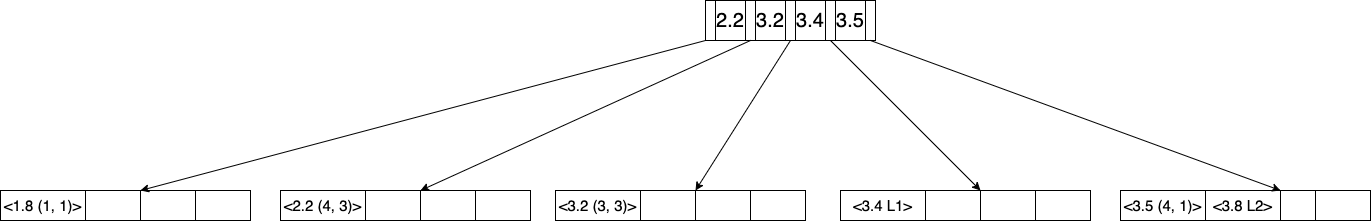
\includegraphics[width=1\textwidth]{img/img3.png}
        \end{center}
    
    \noindent The position of the tuples in the file (page \#, slot \#) are used to identify the different tuples. Note that for practical reasons, when a certain key (GPA) corresponds to a number of distinct entries that is too large, the list is replaced with a variable. List variables definitions are bellow: \\
    L1 = [(1, 3), (1, 4), (2, 1), (2, 2), (2, 3), (2, 4), (3, 1)]\\
    L2 = [(1, 2), (3, 2), (3, 4), (4, 2)]
    
    \item 
            \begin{enumerate}[label={\arabic*.}]
                \item If the tuples in $f$ are sorted, they will appear in the following order:\\
                    <1.8 (1, 1)> \\
                    <2.2, (1, 2)> \\
                    <3.2, (1, 3)> \\
                    <3.4 (1, 4), (2, 1), (2, 2), (2, 3), (2, 4), (3, 1), (3, 2)> \\
                    <3.5 (3, 3)> \\
                    <3.8, (3, 4), (4, 1), (4, 2), (4, 3)> \\
                    \noindent First, the system would need to access the first leaf node with an index value corresponding to the search's criteria (i.e. gpa between 3.0 and 3.5 inclusive). The first value is 3.2 for an entry at page 1 slot 3. Since data is sorted, the system can take advantage of the fact that each node has a bidirectional pointer to the next leaf block. It can keep reading leaf nodes as long as the index value respects the criteria and return the 9 corresponding entries. In total, the system would need to read 3 pages (pages 1, 2, and 3) costing only 1 I/O per page of records thus, 3 I/O. 
                    
                \item If the tuples in $f$ are not sorted, they will appear in the following order:\\
                        <1.8 (1, 1)> \\
                        <2.2, (4, 3)> \\
                        <3.2, (3, 3)> \\
                        <3.4 (1, 3), (1, 4), (2, 1), (2, 2), (2, 3), (2, 4), (3, 1)> \\
                        <3.5 (4, 1)> \\
                        <3.8, (1, 2), (3, 2), (3, 4), (4, 2)> \\
                    \noindent Here, since entries are not sorted in the pages, the system would need to return and read the next index from the index tree before proceeding. This time, we would therefore need at least 1 I/O per record (note that for clustered indexes, it is only 1 I/O per page of records). Since there are 9 entries that respect the criteria, we can expect at least 9 I/O.
                \item We realize that the number of pages accessed tripples  when tuples are unsorted (unclustered indexes) in comparison to when they are sorted (clustered indexes). This factor can quickly increase as the distribution of GPA widen and the number of tuples and tuples per page increases. Also note that clustered indexes are particularly efficient for range searches since it takes advantage of the fact that entries are sorted and can quickly go through pages without having to references the $B^+$-tree each time. However, clustered indexes are more expensive to maintain as files requires periodical sorting as data is added. 
            \end{enumerate}
\end{enumerate}